\documentclass{llncs}\usepackage[]{graphicx}\usepackage[]{color}
%% maxwidth is the original width if it is less than linewidth
%% otherwise use linewidth (to make sure the graphics do not exceed the margin)
\makeatletter
\def\maxwidth{ %
  \ifdim\Gin@nat@width>\linewidth
    \linewidth
  \else
    \Gin@nat@width
  \fi
}
\makeatother

\definecolor{fgcolor}{rgb}{0.345, 0.345, 0.345}
\newcommand{\hlnum}[1]{\textcolor[rgb]{0.686,0.059,0.569}{#1}}%
\newcommand{\hlstr}[1]{\textcolor[rgb]{0.192,0.494,0.8}{#1}}%
\newcommand{\hlcom}[1]{\textcolor[rgb]{0.678,0.584,0.686}{\textit{#1}}}%
\newcommand{\hlopt}[1]{\textcolor[rgb]{0,0,0}{#1}}%
\newcommand{\hlstd}[1]{\textcolor[rgb]{0.345,0.345,0.345}{#1}}%
\newcommand{\hlkwa}[1]{\textcolor[rgb]{0.161,0.373,0.58}{\textbf{#1}}}%
\newcommand{\hlkwb}[1]{\textcolor[rgb]{0.69,0.353,0.396}{#1}}%
\newcommand{\hlkwc}[1]{\textcolor[rgb]{0.333,0.667,0.333}{#1}}%
\newcommand{\hlkwd}[1]{\textcolor[rgb]{0.737,0.353,0.396}{\textbf{#1}}}%

\usepackage{framed}
\makeatletter
\newenvironment{kframe}{%
 \def\at@end@of@kframe{}%
 \ifinner\ifhmode%
  \def\at@end@of@kframe{\end{minipage}}%
  \begin{minipage}{\columnwidth}%
 \fi\fi%
 \def\FrameCommand##1{\hskip\@totalleftmargin \hskip-\fboxsep
 \colorbox{shadecolor}{##1}\hskip-\fboxsep
     % There is no \\@totalrightmargin, so:
     \hskip-\linewidth \hskip-\@totalleftmargin \hskip\columnwidth}%
 \MakeFramed {\advance\hsize-\width
   \@totalleftmargin\z@ \linewidth\hsize
   \@setminipage}}%
 {\par\unskip\endMakeFramed%
 \at@end@of@kframe}
\makeatother

\definecolor{shadecolor}{rgb}{.97, .97, .97}
\definecolor{messagecolor}{rgb}{0, 0, 0}
\definecolor{warningcolor}{rgb}{1, 0, 1}
\definecolor{errorcolor}{rgb}{1, 0, 0}
\newenvironment{knitrout}{}{} % an empty environment to be redefined in TeX

\usepackage{alltt}
\usepackage{listings}
\usepackage{moreverb}
\IfFileExists{upquote.sty}{\usepackage{upquote}}{}
\begin{document}
\title{Problem Set 2}
\author{Thibault Doutre, ID : 26980469}
\institute{STAT 243 : Introduction to Statistical Computing}
\date{}
\maketitle
\bigbreak
\noindent
I worked on my own.
%%%%%%%%%%%%%%%%%%%%%%%%%%%%%%%%%%%%%%%%%%%%%%%%%%%%%%%%%%%
\section{Data processing using bash}
%%%%%%%%%%%%%%%%%%%%%%


Download file.
\begin{lstlisting}[frame=single] 
curl -o data.csv.bz2 "www.stat.berkeley.edu/share/paciorek
/ss13hus.csv.bz2"
\end{lstlisting}
Create script with vim editor.
\begin{lstlisting}[frame=single] 
vim script.sh
\end{lstlisting}
The script contains a function with 4 parameters :
\begin{itemize}
\item arg1 : compressed data (.csv.bz2 format)
\item arg2 : number of random lines to get
\item arg3 : regular expression in order to match the columns we want
\item arg4 : set seed, for reproducibility purposes

\end{itemize}
Algorithm :
\begin{itemize}
\item Set seed.
\item Set the counter variable "var" to zero. It will indicate the position of every field we want to extract.
\item Set the "index" string variable to NULL. This variable will used for the "cut" command. It corresponds to the positions of the fields in the data set.
\item Set IFS to "," for convenience in the "for" loop. The machine will interpret the first line of the file as a list of strings.
\item For every field, do :
\begin{itemize}
\item Increment "var".
\item Make a regular expression in order to state if the selected field is among the ones we want. If it is not the case nothing happens for this step. Otherwise :
\begin{itemize}
\item Add the position of the field to the "index" variable. 
\item Add coma. I differentiate by case when the variable "index" is empty or not in order to avoid beginning with a coma.
\end{itemize}
\end{itemize}
At the end of the loop, "index" looks like "7,12,..." depending on the positions of the fields. We must notice that the list is ordered by index, but it does not matter since variables will be labeled by name.
\item Reset IFS to a space (default value)
\item Put the first line of the file (i.e. the header) to a new file
\item Add 10,000 random lines by doing these steps :
\begin{itemize}
\item Open the csv file
\item Select lines corresponding to the selected fields by using the index variable into the cut command
\item Remove the first line I have already added to the file
\item Shuffle the rows in order to have a random selection
\item Take the first 10,000 rows and add them into the file.
\end{itemize}
\end{itemize}
\noindent
Here is the bash script.

\noindent
\begin{boxedverbatim}
#!/bin/bash

subset_data()
{
# arg1 = compressed data, .csv.bz2 format
# arg2 = number of random lines to get
# arg3 = regular expression
# arg4 = seed

RANDOM=$4
var=0
index=""
IFS=","
for i in $( bzcat $1 | head -1 )
do
        var=$((var+1))
        if [[ "$i" =~ $3 ]]
        then
                if [ -n "$index" ]
                then
                        index=$index$","$var
                else
                        index=$var
                fi
        fi
done
IFS=" "
bzcat $1 | head -n 1 | cut -d',' -f $index > data.subset.csv
bzcat $1 | cut -d',' -f $index | sed '1d' | gshuf | head -$2 >>
data.subset.csv
}
\end{boxedverbatim}
\bigbreak
\noindent
Execute the script with the bash command. This takes approximately 2 minutes and 30 seconds to run on my laptop.
\begin{lstlisting}[frame=single] 
source script.sh ; subset_data data.csv.bz2 10000 "^("ST"|
"NP"|"BDSP"|"BLD"|"RMSP"|"TEN"|"FINCP"|"FPARC"|"HHL"|"NOC"
|"MV"|"VEH"|"YBL")$" 1
\end{lstlisting}
The CSV file of a random sample of 10,000 households containing the following fields for those households: "ST", "NP", "BDSP", "BLD", "RMSP", "TEN", "FINCP","FPARC", "HHL", "NOC", "MV", "VEH" and "YBL" is created.
\section{R code}
I import the dataset from the CSV file. It has only 10,000 rows so it is much easier for R to deal with it now.
\begin{knitrout}
\definecolor{shadecolor}{rgb}{0.969, 0.969, 0.969}\color{fgcolor}\begin{kframe}
\begin{alltt}
\hlkwd{setwd}\hlstd{(}\hlstr{'~/Documents/stat243/ps2'}\hlstd{)}
\hlstd{data}\hlkwb{=}\hlkwd{as.data.frame}\hlstd{(}\hlkwd{read.csv}\hlstd{(}\hlstr{'./data.subset.csv'}\hlstd{))}
\hlkwd{attach}\hlstd{(data)}
\hlkwd{head}\hlstd{(data)}
\end{alltt}
\begin{verbatim}
##   ST NP BDSP BLD RMSP TEN VEH YBL FINCP FPARC HHL MV NOC
## 1 17  1    3   2    6   2   1   5    NA    NA   1  7   0
## 2 32  4    4   2    7   3   1   7 28000     3   1  6   0
## 3 19  1   NA  NA   NA  NA  NA  NA    NA    NA  NA NA  NA
## 4 48  2    3   2    6   2   2   3 66000     4   1  5   0
## 5 48  1    3   2    6   2   1   3    NA    NA   2  7   0
## 6 48  0    3   2    8  NA  NA   5    NA    NA  NA NA  NA
\end{verbatim}
\begin{alltt}
\hlkwd{nrow}\hlstd{(data)}
\end{alltt}
\begin{verbatim}
## [1] 10000
\end{verbatim}
\end{kframe}
\end{knitrout}
\noindent
By calculating the correlation, we can see that NP and NOC have the strongest correlation coefficient among every pairs of variables. It is confirmed when doing a cross-tabulation or plotting the data.

\begin{knitrout}
\definecolor{shadecolor}{rgb}{0.969, 0.969, 0.969}\color{fgcolor}\begin{kframe}
\begin{alltt}
\hlkwd{cor}\hlstd{(}\hlkwd{na.omit}\hlstd{(data)}\hlopt{$}\hlstd{NP,}\hlkwd{na.omit}\hlstd{(data)}\hlopt{$}\hlstd{NOC,}\hlkwc{method}\hlstd{=}\hlstr{"kendall"}\hlstd{)}
\end{alltt}
\begin{verbatim}
## [1] 0.6501196
\end{verbatim}
\begin{alltt}
\hlkwd{table}\hlstd{(NP,NOC)}
\end{alltt}
\begin{verbatim}
##     NOC
## NP      0    1    2    3    4    5    6    7    8   11
##   0     0    0    0    0    0    0    0    0    0    0
##   1  2278    0    0    0    0    0    0    0    0    0
##   2  2767  181    0    0    0    0    0    0    0    0
##   3   639  522  109    0    0    0    0    0    0    0
##   4   247  167  606   43    0    0    0    0    0    0
##   5    99   62   84  219   14    0    0    0    0    0
##   6    31   11   19   32   54    3    0    0    0    0
##   7    14   10    7   10    8   20    1    0    0    0
##   8     8    3    4    2    3    4    4    0    0    0
##   9     5    2    3    2    1    1    0    1    0    0
##   10    0    0    0    1    0    0    1    0    1    0
##   11    2    1    0    0    0    0    1    0    0    0
##   12    0    0    0    1    0    1    0    0    0    0
##   13    0    0    0    0    1    0    0    0    0    0
##   14    0    0    0    0    0    0    0    0    0    1
\end{verbatim}
\begin{alltt}
\hlkwd{plot}\hlstd{(NP,NOC,}\hlkwc{main}\hlstd{=}\hlstr{"NOC versus NP, cor ~= 73%"}\hlstd{)}
\end{alltt}
\end{kframe}
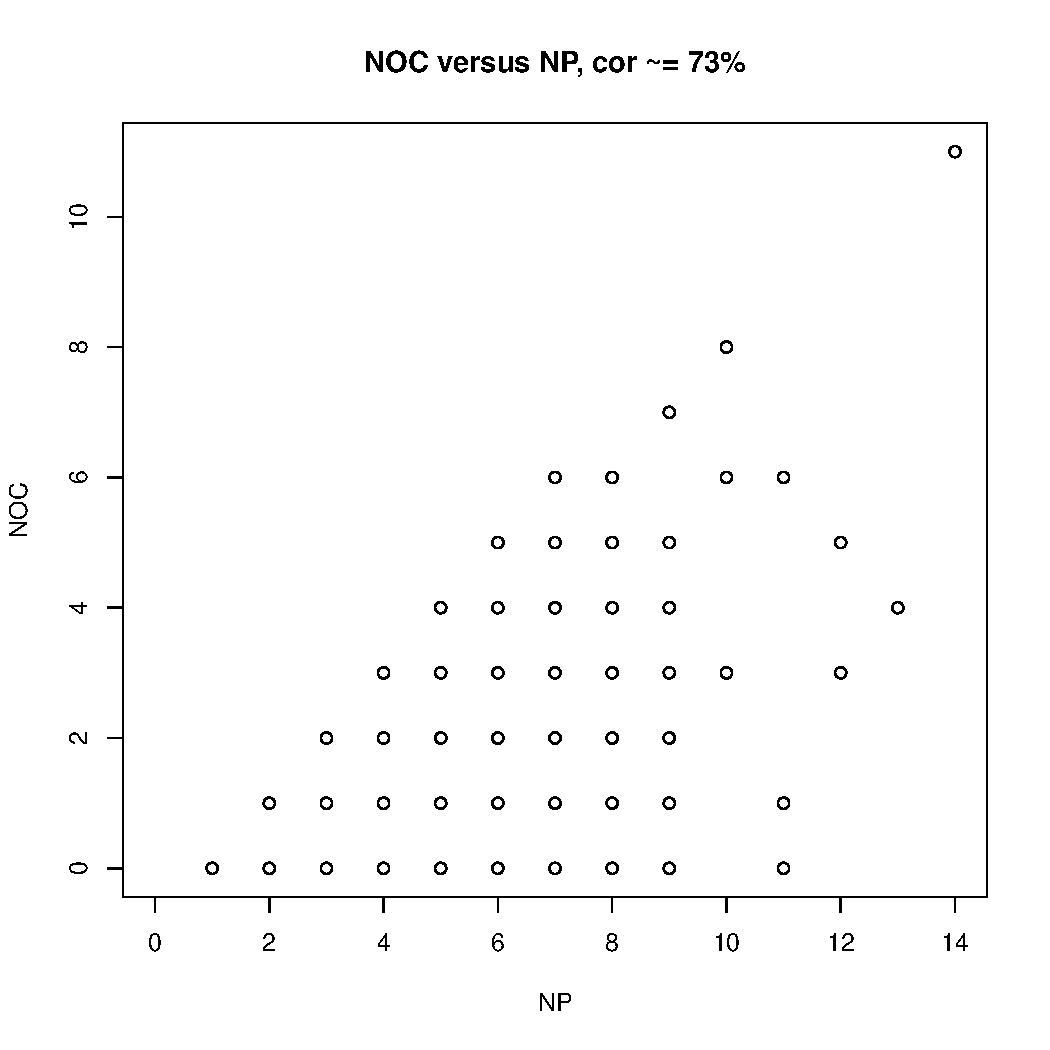
\includegraphics[width=\maxwidth]{figure/unnamed-chunk-2-1} 

\end{knitrout}
\section{Time complexity}
Once the bzfile downloaded, the bash script takes approximately 2 minutes and 30 seconds to run on my computer. I think it is more than fair. I could have been much faster by taking the first rows of the dataset with the "head" command. But in this case, I would have not taken random lines on the whole dataset.
As for the R commands, they run in less than a second because it only reads 10,000 rows and a few columns.

\section{Comparison between scan() and read.csv()}
We obtain better results with opening a file with scan than read.csv. To get better results, we can bzip the file, open a connection to the compressed file and then use scan. However, when trying to compute these two functions to the whole compressed data file, it takes a very long time compared to the required time for the bash script to run.
\begin{knitrout}
\definecolor{shadecolor}{rgb}{0.969, 0.969, 0.969}\color{fgcolor}\begin{kframe}
\begin{alltt}
\hlkwd{setwd}\hlstd{(}\hlstr{'~/Documents/stat243/ps2'}\hlstd{)}
\hlstd{con}\hlkwb{=}\hlkwd{file}\hlstd{(}\hlstr{'./data.subset.csv'}\hlstd{)}
\hlkwd{system.time}\hlstd{(}\hlkwd{read.csv}\hlstd{(con))}
\end{alltt}
\begin{verbatim}
##    user  system elapsed 
##   0.066   0.002   0.069
\end{verbatim}
\begin{alltt}
\hlstd{con}\hlkwb{=}\hlkwd{file}\hlstd{(}\hlstr{'./data.subset.csv'}\hlstd{)}
\hlkwd{system.time}\hlstd{(}\hlkwd{scan}\hlstd{(con,}\hlkwc{what}\hlstd{=}\hlstr{"integer"}\hlstd{,}\hlkwc{sep}\hlstd{=}\hlstr{","}\hlstd{))}
\end{alltt}
\begin{verbatim}
##    user  system elapsed 
##   0.054   0.000   0.055
\end{verbatim}
\begin{alltt}
\hlkwd{close}\hlstd{(con)}
\end{alltt}
\end{kframe}
\end{knitrout}

\end{document}
